\documentclass[12pt, twoside]{article}
\usepackage[francais]{babel}
\usepackage[T1]{fontenc}
\usepackage[latin1]{inputenc}
\usepackage[left=7mm, right=1cm, top=1cm, bottom=7mm]{geometry}
\usepackage{float}
\usepackage{graphicx}
\usepackage{array}
\usepackage{multirow}
\usepackage{amsmath,amssymb,mathrsfs}
\usepackage{soul}
\usepackage{textcomp}
\usepackage{eurosym}
 \usepackage{variations}
\usepackage{tabvar}

\begin{document}


\section*{\center{Aide individualis�e: Fonction croissante et d�croissante}}

\subsection*{Exercice 1}

Dessiner deux courbes diff�rentes tels que la fonction associ�e ait le tableau
de variation suivant:
\[\begin{tabvar}{|C|CCCCCCC|} 
  \hline
  x &-6 & &2 & &3 & &4\\ 
  \hline
  \niveau{2}{3}f(x)
  &4 &\decroit
  &0 &\croit 
  &3 &\decroit& -6
 \\ \hline
  \end{tabvar}\]
 
\medskip
 

\begin{tabular}{cc}
\begin{minipage}{9cm}
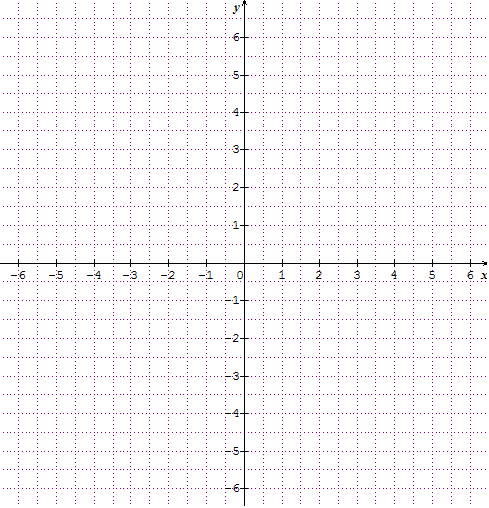
\includegraphics[width=8cm]{images/repere.png}
\end{minipage}
&
\begin{minipage}{9cm}
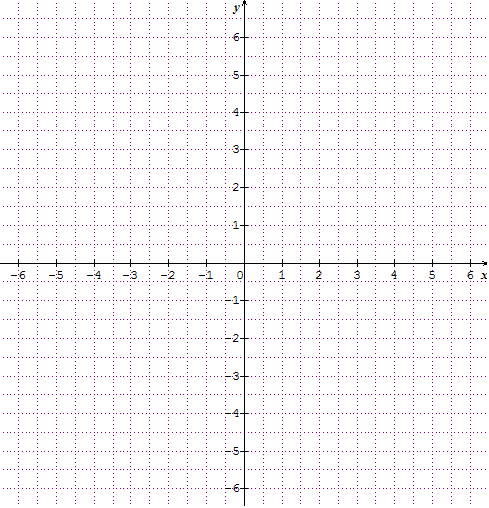
\includegraphics[width=8cm]{images/repere.png}
\end{minipage}
\end{tabular}



\subsection*{Exercice 2}

\begin{tabular}{cc}
\begin{minipage}{6cm}
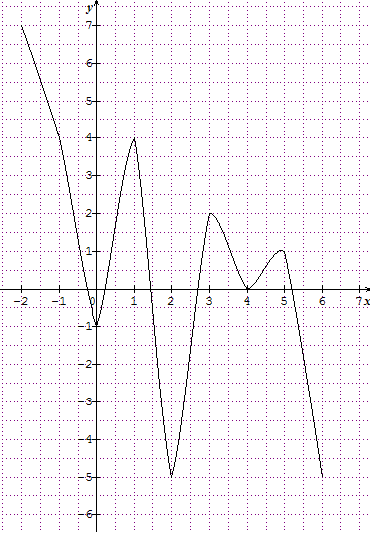
\includegraphics[width=6cm]{images/ex2.png}
\end{minipage}
&
\begin{minipage}{12cm}
D�crire les variations de la
fonction repr�sent�e graphiquement. Dresser son tableau de variation.
\end{minipage}
\end{tabular}

\bigskip

\bigskip

\bigskip

\bigskip

\bigskip

\subsection*{Exercice 3}

Soit $f$ une fonction d�finie sur $]-\infty;4]$ dont le tableau de variation est
le suivant: \[\begin{tabvar}{|C|CCCCCCC|} 
  \hline
  x &-\infty & &-1 & &2 & &4\\ 
  \hline
  \niveau{2}{3}f(x)
  & &\decroit
  &0 &\croit 
  &3 &\decroit& -7
 \\ \hline
  \end{tabvar}\]

\begin{enumerate}
  \item Comparer les nombres suivants lorsque cela est possible:

 $f(-3)$ et $f(-2)$:
 
 $f(0)$ et $f(1)$:
 
 $f(-6)$ et $f(2,7)$:
 
 $f(0,5)$, $f(0,51)$ et $f(0,52)$:
 
 $f(-2)$ et $f(4)$:
 \item Quel est le signe de $f(x)$ pour $x<-1$?
 
 \enskip
 
 \item Quel est le minimum de la fonction $f$? Pour quelle valeur est-il
 atteint?
 
 \enskip
 
 \item Peut-on conna�tre le maximum?
 \item Peut-on avoir $f(3)=-8$? $f(3)=4$? Donner un encadrement de $f(3)$.
 
 
\end{enumerate}

\bigskip

\bigskip

\subsection*{Exercice 4}


Soit 
\begin{minipage}{3cm}

\begin{align*}
f: \ & ]0;+ \infty[\  \rightarrow \ \mathbb{R} \\
& x \ \mapsto \  \dfrac{3}{x}+2
\end{align*}
\end{minipage}



Montrer que la fonction $f$ est d�croissante sur $[0;+\infty[$.



\end{document}
